%%%%%%%%%%%%%%%%%%%%%%%%%%%%%%%%%%%%%%%%%%%%%%%%%%%%%%%%%%%%%%%%%%% 
%                                                                 %
%                            CHAPTER                              %
%                                                                 %
%%%%%%%%%%%%%%%%%%%%%%%%%%%%%%%%%%%%%%%%%%%%%%%%%%%%%%%%%%%%%%%%%%% 

\chapter{Parallel Fixed Size Least Square Support Vector Machines in Action }
\section{Introduction}
This chapter describes the actual testing done on the parallel version of Fixed Size Least Square Support Vector Machines.
The different tests are described as well as why they are necessary.
An hypothesis for each test is made with a reasonable explanation.
The test results are presented and a conclusion about the test process ends this chapter.\footnote{This is not a conclusion of the general objectives that were stated.}
\section{What To Test}
For all the testings we use two different data sets.
The first dataset is considered small to medium size, consisting of the following characteristics:
\begin{itemize}
	\item Title: Concrete Compressive Strength\cite{UCIMachi66:online}
	\item Number of attributes: 9
	\item kernel type: RBF kernel
	\item Number of data points: 1030
	\item Type: function estimation
\end{itemize}
With a size of 1030 elements, this data sets allows execution on a personal computer.
This is important to do initial testing and set base characteristics of the behaviour.
\par 
The second data set has the following characteristics:
\begin{itemize}
	\item Title: YearPredictionMSD Data Set\cite{UCIMachi93:online}
	\item Number of attributes: 90
	\item Kernel type: RBF kernel
	\item Number of data points: 515345
	\item Type: function estimation
\end{itemize}
With a size of more than 500 000 data points and more than 50 attributes this can be considered a, so called, big data set.
It is still possible to execute the algorithm with this data set on a personal computer but the performance will decrease drastically.
\par 
To make adequate performance conclusions, multiple tests need to be completed.
A base indicator of computing time is found by executing both data sets on a personal computer in a non parallel matter.
These results will not have any meaning in the final conclusion but give a good indication of the computational time we are dealing with.
\par 
The serious tests will be done on a much more powerfull machine. 
In the original objective a HPC was mentioned as a host machine.
As described in the literature review, the term HPC is very vague and can include multiple types of machines.
I decided to use the service based approach\footnote{This is as well described in the literature review.}.
NVIDIA supports Matlab cloud computing with Amazon Web Services.
This is done using an ubuntu virtual machine on the AWS servers, connected to both a powerful CPU and GPU.
The virtual machine runs a Matlab docker container.\cite{MATLABDe46:online}
This specific setup and docker container is called MATLAB Deep Learning Container on NVIDIA GPU Cloud.
The hardware specifics are shown in figure~\ref{fig:awsspec}.
\begin{figure}[H]
	\centering
	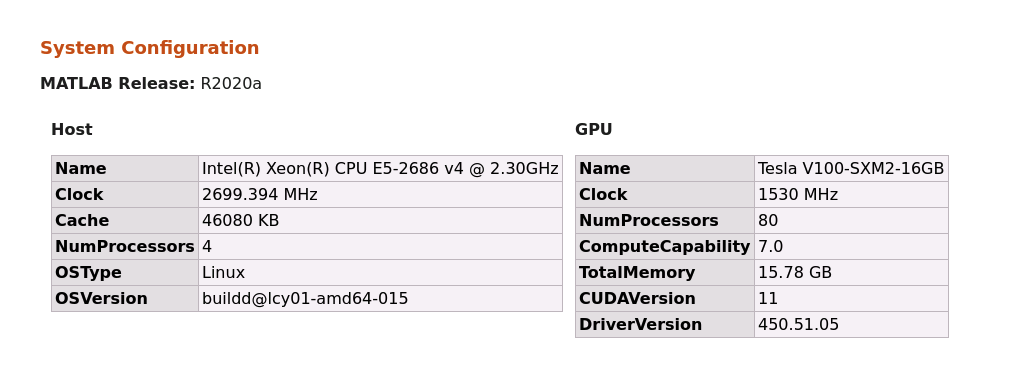
\includegraphics[width=\linewidth]{awsSpecifications.png}
	\caption{The hardware specifications of the test bench used in the MATLAB Deep Learning Container on NVIDIA GPU Cloud.}
	\label{fig:awsspec}
\end{figure}
In the appendices chapter, this setup is discussed with more details.
\par 
On this test bench setup, both data sets need to be tested in both sequential and parallel execution to achieve representative performance results.
\subsection{Sequential}
The sequential execution is needed to set a base mark.
Without a base mark, execution times of parallel code blocks will not have any meaning. 
\subsubsection{On Device Execution}
The on device sequential test with the small dataset has the following characteristics:
\begin{itemize}
	\item Title: Concrete Compressive Strength\cite{UCIMachi66:online}
	\item Number of attributes: 9
	\item Kernel type: RBF kernel
	\item Number of support vectors: [10, 50, 100, 300, 700, 730]
	\item Number of folds: 10
	\item SV selection stop after $N/20$ unsuccessful operations.
	\item Starting $\sigma$= 0.75
	\item Times of execution: 25
\end{itemize}
The on device sequential test with the large dataset has the following characteristics:
\begin{itemize}
	\item Title: YearPredictionMSD Data Set\cite{UCIMachi93:online}
	\item Number of attributes: 90
	\item Kernel type: RBF kernel
	\item Number of support vectors: 730
	\item Number of folds: 10
	\item SV selection stop after $N/10000$ unsuccessful operations.
	\item Starting $\sigma$= 0.75
	\item Times of execution: 1
\end{itemize}
This test is only going to be executed once because the data set is so large and the execution time on my personal device is not going to be representative for performance comparison.
\subsubsection{HPC execution}
The HPC sequential test with the small dataset has the following characteristics:
\begin{itemize}
	\item Title: Concrete Compressive Strength\cite{UCIMachi66:online}
	\item Number of attributes: 9
	\item Kernel type: RBF kernel
	\item Number of support vectors: [10, 50, 100, 300, 700, 730]
	\item Number of folds: 10
	\item SV selection stop after $N/20$ unsuccessful operations.
	\item Starting $\sigma$= 0.75
	\item Times of execution: 25
\end{itemize}
The HPC sequential test with the large dataset has the following characteristics:
\begin{itemize}
	\item Title: YearPredictionMSD Data Set\cite{UCIMachi93:online}
	\item Number of attributes: 90
	\item Kernel type: RBF kernel
	\item Number of support vectors: [700, 1500, 2000, 2500]
	\item Number of folds: 10
	\item SV selection stop after $N/10000$ unsuccessful operations.
	\item Starting $\sigma$= 0.75
	\item Times of execution: 25
\end{itemize}
This test is going to be executed 25 times to achieve good base results for the sequential execution times for multiple numbers of support vectors.
\subsection{Parallel}
The parallel testing is done on slightly altered code. 
All the candidates defined in chapter 4 are coded in the correct manner.
In the appendices is shown how parallel executable code is written in Matlab.
\subsubsection{On Device Execution}
On device parallel test is not possible due to a lack of CUDA support.
In the entirely this does not matter because the real comparison is made between sequential an parallel execution on the HPC.
However this directly point to the restriction of GPU parallel computing as described in the literature review.
\subsubsection{HPC Execution}
The HPC parallel test with the small dataset has the following characteristics:
\begin{itemize}
	\item Title: Concrete Compressive Strength\cite{UCIMachi66:online}
	\item Number of attributes: 9
	\item Kernel type: RBF kernel
	\item Number of support vectors: [10, 50, 100, 300, 700, 730]
	\item Number of folds: 10
	\item SV selection stop after $N/20$ unsuccessful operations.
	\item Starting $\sigma$= 0.75
	\item Times of execution: 25
\end{itemize}
The HPC parallel test with the large dataset has the following characteristics:
\begin{itemize}
	\item Title: YearPredictionMSD Data Set\cite{UCIMachi93:online}
	\item Number of attributes: 90
	\item Kernel type: RBF kernel
	\item Number of support vectors: [700, 1500, 2000, 2500]
	\item Number of folds: 10
	\item SV selection stop after $N/10000$ unsuccessful operations.
	\item Starting $\sigma$= 0.75
	\item Times of execution: 25
\end{itemize}
This test is going to be executed 25 times to achieve good base results for the parallel execution times for multiple numbers of support vectors.
\section{What To Measure}
The decision is made to measure the complete execution time.
This is a good indicator because it provides a total speed-up of the algorithm. 
The following things have to be taken into account:
\begin{itemize}
	\item The dataset will be loaded into Matlab every time. Relevant because this is a sequential task that is always going to be a bottleneck even when every detail of the algorithm is optimized.
	\item The SV Selection is also part of the time measurement. Relevant because: however the fact that it is mostly a sequential task, it does call the kernel matrix function which is parallelized, and it is a major part of the algorithm that contributes to the total performance characteristic of the FS LS-SVM algorithm.
\end{itemize}
\section{Hypothesis}
Knowing that copying data to and from the GPU dedicated memory creates extra overhead and that the Intel Xeon processor is quiet powerful, I suspect that matrix computations and alterations with small dimensions are not going to lead to a performance increase.
Translating this to my test cases: I do not expect an execution time speed up for the small data set comparing parallel and sequential execution on the HPC.
I suspect larger execution times for small number of support vectors and at the same time much better results for large number of support vectors.
Somewhere is going to be a critical point where it becomes beneficial to use the parallel execution.
Because of the fact that Matlab uses optimization on the CPU and that the HPC CPU is quiet powerful, I suspect the critical point to be just higher than the max amount of support vectors in the small data set (higher than 700). 
An exact speed-up prediction number is hard to calculate because that is very dependent on the following items:
\begin{itemize}
	\item GPU frequency (known)
	\item GPU percentage of used GPU cores for computations (hard tot calculate and very data set specific)
	\item Data transfer speed (unknown)
	\item CPU multi core optimization (unknown, hard to quantify) 
	\item CPU frequency (known)
	\item Exact percentage of parallel code (estimation possible but not exact)
	\item Overhead with CPU execution when main memory elements have to be swapped (impossible to predict/calculate)
\end{itemize}
Because of the fact that the \textit{fast $v$ fold crossvalidation} algorithm is called so many times in this algorithm, a large number of data transfers is needed.
The impact of the needed time, and overhead created for cpu to manage this transfer is out of my knowledge to calculate and most important will have a significant impact on the total execution time when executing code in parallel.
This results in the fact that the equation of Amdahls' law\ref{eq:amadahl} cannot provide us with a representative result
Therefore I double down on the hypothesis made earlier that not all test cases are going to result in a speed up because of the hard calculate overhead and hard to quantify already present optimization of the available CPU cores by Matlab.\footnote{In case of Intel processors Matlab is using intel mkl for blas optimization}
\section{Test Results}
\subsection{Problems}
When starting the execution of the different tests, problems occurred in the \textit{fast $v$ fold crossvalidation} function.
As described in chapter 4, this section exists of a nested CPUparallel region with both in and before the second region multiple GPUparallel computations.
The parallel computing toolbox does not provide the same amount of control compared to C++ frameworks for multithreading\footnote{Hence the initial choice for C++ and OpenMP.}.
Matlab struggles interpreting variables, especially in combination with GPU combined usage.
On top of that, with large data sets and large numbers of support vectors, the used amount of memory on the GPU rises quickly, when in that case multiple pool workers (CPU threads) call the GPU for dedicated matrix computations a bottleneck in GPU memory rises.
When making use of 700 or more support vectors, CPU parallel execution of the $J$ couples and $v$ folds of the \textit{fast $v$ fold crossvalidation} algorithm became impossible, even on the NVIDIA Tesla v-100 GPU.
Therefore alterations were made to execute $J$ couples and $v$ folds sequential while maintaining the GPU parallel execution for all other regions as described in table~\ref{tab:parcandidates}.
\subsection{Results After Alteration}
As described in this chapter, every test on the HPC is run at least 25 times for every tested number of support vectors to get a stable result.
The mean of the execution time is calculated for every number of support vector used.
The results for the small data set can be found in table~\vref{tab:resultssmall} and shown in figure~\ref{fig:smallresult}.
\begin{table}[]
	\centering
	\begin{tabular}{l|llllll}
		Number of SV 		& 10          	& 50         & 100         & 300        & 700       & 730    \\ \hline
		On device Sequential [s]   	& 0,732  	   	& 1,090  	 & 2,104 	   & 9,809 	& 52,628 	& 55,696 \\
		HPC Sequential [s]   	& 0,676  	   	& 1,455  	 & 2,465 	   & 10,367 	& 39,686 	& 42,621 \\
		HPCParallel   [s]  	& 4,661  	   	& 5,236  	 & 6,082  	   & 16,257 	& 30,528  	& 29,991 \\ \hline
		HPC Seq/Par      		& 0,144  	   	& 0,278	     & 0,405	   & 0,637 		& 1,300 	& 1,421
	\end{tabular}
	\caption{Small data set results: the mean execution times in seconds for every number of support vectors, Seq/par row shows the corresponding speed-up factor.}
	\label{tab:resultssmall}
\end{table}
The results for the large data set can be found in table~\vref{tab:resultslarge}.
\begin{table}[]
	\centering
	\begin{tabular}{l|lll}
		Number of SV       & 700      & 1500     & 2000 		\\ \hline
		On device Sequential [s] & 2854,697 & / &  /    \\
		HPC Sequential {[}s{]} & 2295,078 & 6863,830 &  9504,194    \\
		HPC Parallel {[}s{]}   & 119,970  & 547,007  &  1064.495	 \\ \hline
		HPC Seq/Par            & 19,130   & 12,548   &  8,928   			
	\end{tabular}
\caption{Large data set results: the mean execution times in seconds for every number of support vectors, Seq/par row shows the corresponding speed-up factor.}
\label{tab:resultslarge}
\end{table}
\begin{figure}
	\centering
	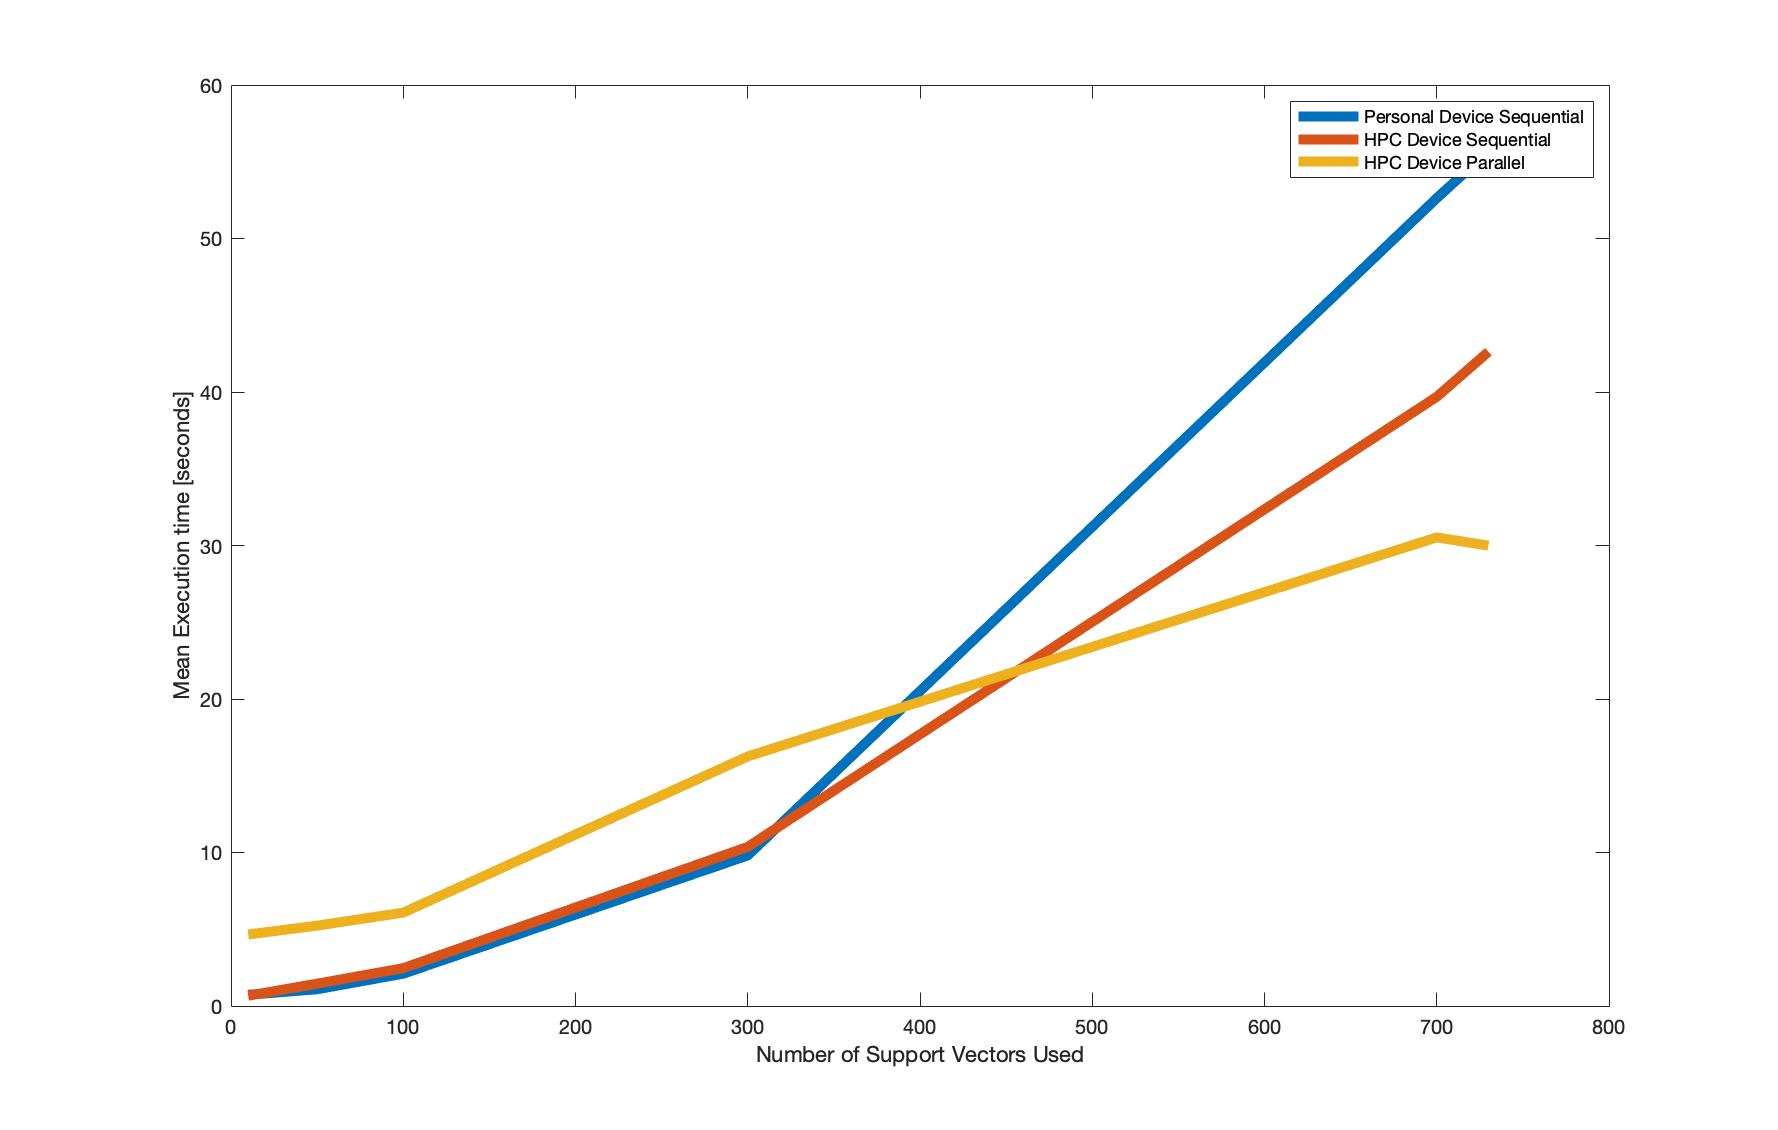
\includegraphics[width=\linewidth]{smallresult.png}
	\caption{Mean values of the execution times on the small data set.}
	\label{fig:smallresult}
\end{figure}
\section{Conclusion}
When looking at the results and taking into account the hypothesis made, a few things stand out.
First, as stated the overhead introduced by copying data back and forth from the main memory to GPU dedicated memory combined with the optimized execution on th CPU does result in worse parallel execution times for a low amount of support vectors.\par 
Looking at the results of the small data set this really stands out for 10, 50 and 100 support vectors.
Resulting in a corresponding speed up factor of way below one. 
What stands out is that the tipping point, where parallel execution becomes interesting is locates at an amount of support vectors below 700.
Because of the power of the CPU this is something I did not expect.\par 
Looking at the results of the large data set, the speed-up factor even for 700 support vectors is way higher compared to the small data set.
The reason behind this has to do with the all the computations done in the FS LS-SVM algorithm.
As described earlier, most operations are with matrices of size $m$\footnote{$m$ stands for the number of support vectors}, but at some points the full data set is still taken into account.\footnote{(Extended) Feature matrix computation and more}.
This results in the fact when dealing with a large dataset the benefit of using GPUparallel execution is going to be larger than with a smaller dataset even when using the same amount of support vectors.





